\documentclass[11pt]{article}
\usepackage{graphicx} % Required for inserting images
\usepackage{indentfirst}
\usepackage{caption}
\usepackage{subfig}
\title{Classifying Obesity Using Multiple Models}
\author{Aadhi Aravind, Nandhana Selvam, Leo Wang, Patrick Manson}
\date{14 March 2024}
\usepackage{geometry}
\geometry{margin= 1in}
\begin{document}

\maketitle

\section{Outline}
    Approximately 1 in 8 people in the world now live with obesity$^{9}$ with numbers projected to continually increase raising concern for one of the globe's biggest health crises. In this document, we analyze the Estimation of Obesity Levels Based On Eating Habits and Physical Condition dataset$^{4}$ to create a model to predict what level of obesity a person is at (if at all) to increase their health awareness and if they should make lifestyle changes or not. The dataset was created by  Fabio Mendoza Palechor and Alexis De la Manotas in 2019, and was oversampled using SMOTE. After performing some basic data analysis and pre-processing the data using a min-max scaler, we decided on three different models we wanted to create. To determine the best one, we analyzed the accuracy of each. First, we developed a Multi-Layer Perceptron and performed hyperparameter tuning, but found that the overall accuracy was solid but could be better. Then, we developed a Deep Neural Network, which created good results as well. Finally, to test if a decision tree-based model would be better we created an Extreme Gradient Boost Model(XGBoost), which when paired with early stopping, created the best model with an accuracy of 97.63\%. We also found that even after performing a k-folds cross-validation of 10, it kept a high accuracy of 95\%. Furthermore, we found that it had high precision and accuracy, which leads us to believe that it should predict obesity levels without any issues. After verifying these issues, we ultimately created a front-end where users can input their data to see where our model places them.
\section{Introduction}

    Obesity is a prevalent issue in the world today and is projected to get worse in the near future with a Lancet study citing that “obesity is now a greater threat to global health than hunger”.$^{1}$ Obesity is defined as having a body mass index (BMI) greater than 30 kilograms per meter squared. The amount of people affected by obesity is anticipated to “rise from 14\% to 24\% of the population”$^{2}$ from 2020 to 2035, which means around 2 billion adults, children, and adolescents will be obese in 2035. Another issue lies in how the steepest increase in obesity is in children and adolescents during this same time period where 20\% of boys and 18\% of girls would be obese in 2035.$^{2}$
	
	Obesity has many negative effects on the body leading to problems like high blood pressure, Type 2 diabetes, stroke, coronary heart disease, and mental illness.$^{3}$ Therefore, obesity is an alarming issue that needs to be prevented. There is no medicinal cure for obesity, unfortunately, but rather people have to change their lifestyle by being more active and eating a healthy diet which requires strong commitment and a clear goal set in mind. 

 Awareness is key in solving the obesity crisis as people should know where they stand since with this knowledge, they can identify if they need to change their lifestyle and what specifically they need to change, be it eating habits or exercise or both. For example, if someone is classified as Overweight then they know that even though they are not obese there is a possibility in the future if they continue with their current lifestyle, so they can start to take preventative measures. This way, the number of people who become obese will reduce as people are more conscious about their health. 

The goal of our project is to accurately classify individuals into levels of obesity based on various factors, such as their eating habits and physical condition, as well as providing preventative measures so that they can improve their health, which is added to the front-end output. The measures must cater to the individual because everyone should be able to use the model and make changes to their specific lifestyle rather than getting feedback that may not affect them. 

The Estimation of Obesity Levels Based On Eating Habits and Physical Condition Dataset$^{4}$ is used in this project focuses on Mexico, where “32.3\% of men and 41\% of women are obese”, Peru, where “21.3\% of men and 26.6\% of women are obese”, and in Colombia, where “29.4\% of men and 12.6\% of women are obese.”$^{5}$ From these statistics, it is an alarming issue in these countries and one that should be approached with caution in the near future. 

\section{Literature Review}
The literature review provides insight into how other people have used the dataset and other similar datasets to predict obesity in the past. When analyzing each paper, the critical aspects include understanding their methodology, why they chose their dataset, to see if any aspects that could be further improved upon, and to find any inspiration for our project. 

\subsection{Predicting risk of obesity and meal planning to reduce the obese in adulthood using artificial intelligence$^{6}$}
Kaur et al. used the same dataset and focused on outputting meals that help reduce obesity in adulthood by checking obesity levels. The study also used a meal planning dataset in conjunction with the meals aspect of their research. Their methodology of their project included preprocessing the data using scaling and converting categorical data to continuous values, and running various models including Bagging algorithms and Boosting algorithms. Models were compared using classification metrics like accuracy, precision, recall, and F-1 score, while also checking performance against different train/test splits. One of the algorithms used was the XGB algorithm which performed the best in all of the classification metrics, making it a very viable option to try in our project. 
\subsection{A Hybrid Machine Learning Model for Estimation of Obesity Levels$^{7}$}


Choudhuri used the same dataset in their project and created a hybrid machine learning model to estimate obesity levels. Choudhuri used a Multilayer Perceptron model and an XGBoost model in conjunction where the multilayer perceptron creates an embedding that is inputted into the XGB model. This hybrid model showcased excellent precision and recall at 99.4\% outperforming the Random Forest model they were comparing with. The hybrid model also outperformed the non-hybrid XGBoost model. The study also addresses the lack of generalization the model may have since it focuses solely on the three countries of the dataset, which is a point of interest in the future. The promising results of the MLP and XGBoost model played a part in our choice of these two models for our project.
\subsection{A Deep Learning Neural Network to Classify Obesity Risk in Portuguese Adolescents Based on Physical Fitness Levels and Body Mass Index Percentiles: Insights for National Health Policies$^{8}$}

Forte et al. utilized a deep neural network with a different dataset that identified the risk of obesity in Portuguese adolescents based on their BMI and physical fitness levels. The neural network had an accuracy of 75\% and K-Folds cross-validation accuracy of 71\%. Since the dataset was fairly small at around 654 data points, cross-validation was used to further validate the results of the small dataset and test how well the model performed on various folds of the dataset. Therefore, since the obesity dataset used in our project is also fairly small with around 2200 data points, cross-validation should be utilized to ensure the model is generalized over the whole dataset.
\subsection{Takeaways}
The main takeaways from the literature review include incorporating the Multilayer Perceptron, XGBoost, and cross-validation into our project. Additionally, the common methodology of all the papers includes preprocessing the data through scaling and then running the models was one that we chose to follow. 

\section{Dataset Description}
We will be using the Estimation of Obesity Levels Based On Eating Habits and Physical Condition$^{4}$ dataset, which was created by Fabio Mendoza Palechor and Alexis De la Hoz Manotas in 2019. The dataset consists of 17 features and 2111 observations from people in Mexico, Peru, and Colombia. There are seven different classification labels which include Insufficient/Under weight, Normal weight, Overweight level I, Overweight level II, Obesity level I, Obesity level II, Obesity level III. 

They generated this dataset through a combination of generating synthetic data using the weka tool and the SMOTE filter, which supplements the data collected from users on a web platform, with a ratio of 77\% synthetic data and 23\% collected data. They collected multiple variables, which include general information about the subject (age, gender, height, weight, family history with overweight); lifestyle information (normal form of transportation, use of technology, smoking, exercise amount); and eating habits (frequency of eating high caloric food, frequency of eating vegetables, amount of meals in a day, consumption of alcohol, consumption of water, calorie tracking, and eating food between meals). The dataset is balanced so there a similar amount of records in each obesity level category which saves us a step of pre-processing. (Refer to Figure 1)

\begin{figure}[h]
    \centering
    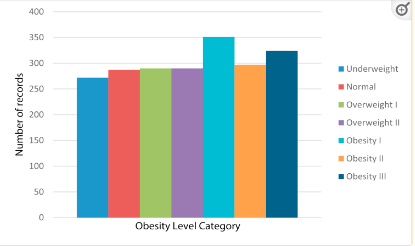
\includegraphics[width=0.5\linewidth]{balancedDataPic.png}
    \captionsetup{font=small}
    \caption{Shows the number of data points for each obesity level category highlighting the balance. Credit:$^{4}$}
    \label{fig:enter-label}
\end{figure}

\section{Proposed Solution}
    \subsection{Methodology}
    Our methodology includes preprocessing the dataset and running the dataset into three different models, comparing classification metrics, including accuracy, precision, and recall. Specifically, we looked at a Multi-Layer Perceptron (MLP), a Deep Neural Network (DNN), and what's known as an eXtreme Gradient Boosting (XGBoost) model. Each model was chosen for its ability to recognize complex patterns and the literature review provided evidence of their good performance. The goal is to identify the model that performs the best in all metrics and doesn’t show any signs of underfitting and overfitting.(Refer to Figure 2)
    \begin{figure}[h]
        \centering
        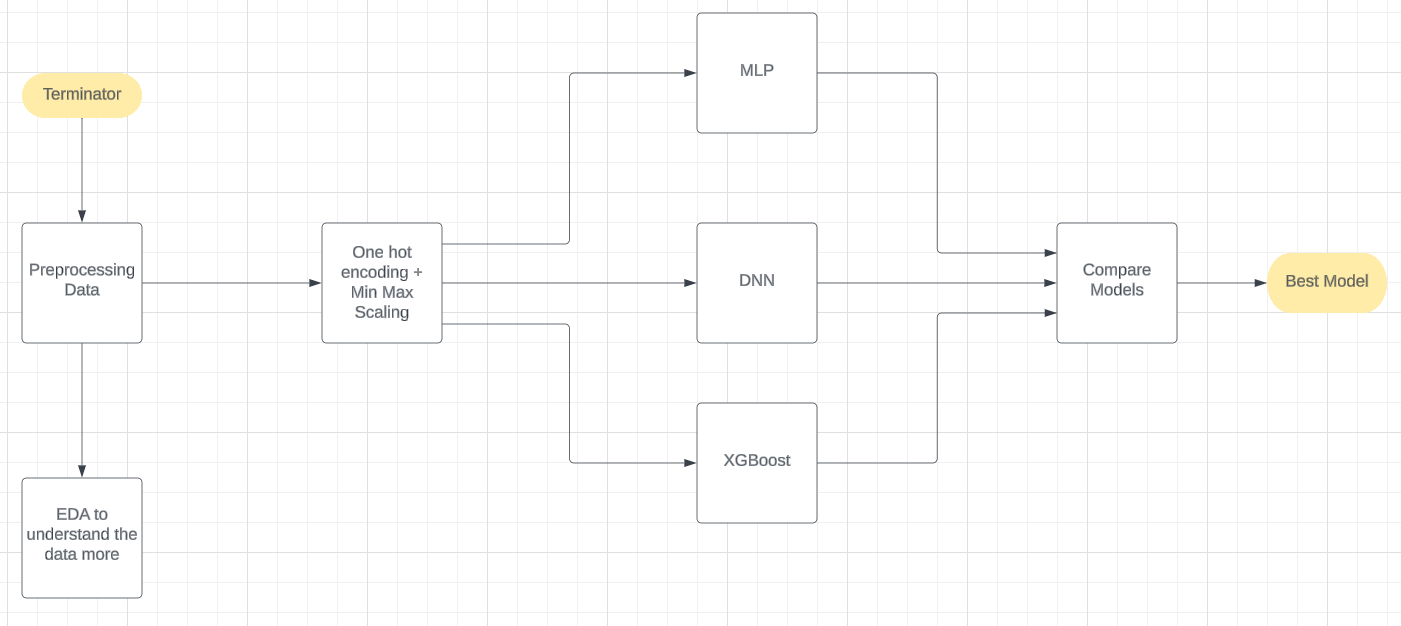
\includegraphics[width=0.9\linewidth]{method.png}
        \caption{Methodology followed}
        \label{fig:enter-label}
    \end{figure}
    \subsection{Preprocessing the Data}
    There are eight features that have categorical data that need to be converted to continuous variables. We used one-hot encoding to remove any bias of a possible ordinal relationship in the categorical variables. Then, with all the data being one-hot encoded, we ran exploratory data analysis to better understand the type of data we are working with and what exactly to look for. 
    
    Our exploratory data analysis began with a correlation matrix. Since the matrix was made after one-hot encoding, the categorical variables have been split up into separate columns. By observing the last seven columns that correspond to the seven different obesity levels, it is evident that weight plays a significant role in predicting obesity across the majority of levels. Other variables with high correlation values include CAEC(consumption of food between meals), family history with overweight, and gender. We can expect that these variables will play a significant role in the classification task. 

    
    We also considered a pair plot in our exploratory data analysis. The weight column has the most clear and distinct patterns. This further proves that weight is an influential variable and is very informative in predicting obesity. Analyzing the weight column shows a clear, linear relationship between the height and weight variables. Thus, weight and height are likely the most helpful in identifying the classes from one another. 
    
    Finally, we can further examine the weight variable in a box plot. As the level of obesity increases, the mean weight also increases, once again indicating a clear connection between weight and obesity levels. The plots are also relatively symmetric with Obesity Type III being the most right skewed. A few outliers are present for Overweight Level II, Obesity Type II, and Obesity Type III as well.
   \begin{figure}[h]
      \centering
      \subfloat[Correlation Matrix with Weight]{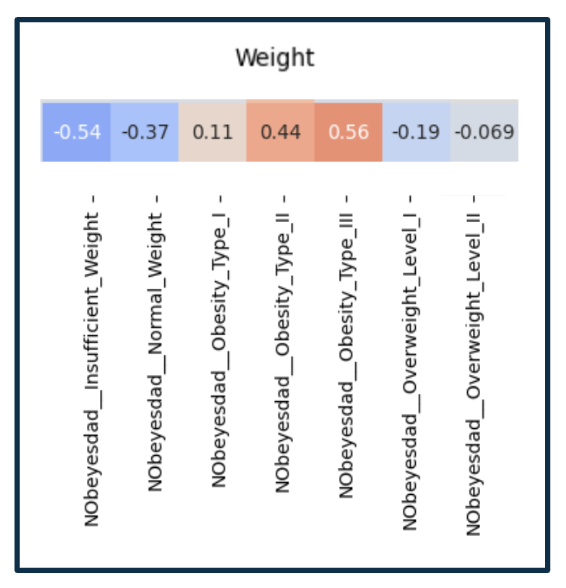
\includegraphics[width=0.2\textwidth]{heatmap.png}\label{fig:f1}}
      \hfill
      \subfloat[Pair Plot between Height and Weight]{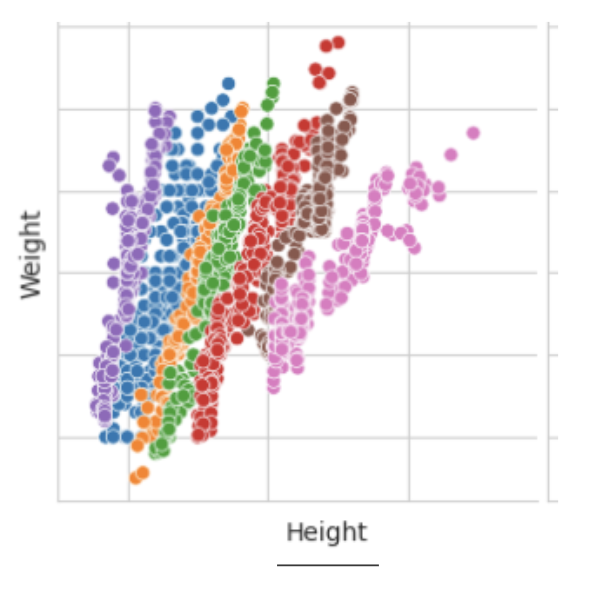
\includegraphics[width=0.3\textwidth]{pairplot.png}\label{fig:f2}}
      \subfloat[Boxplot with weight]{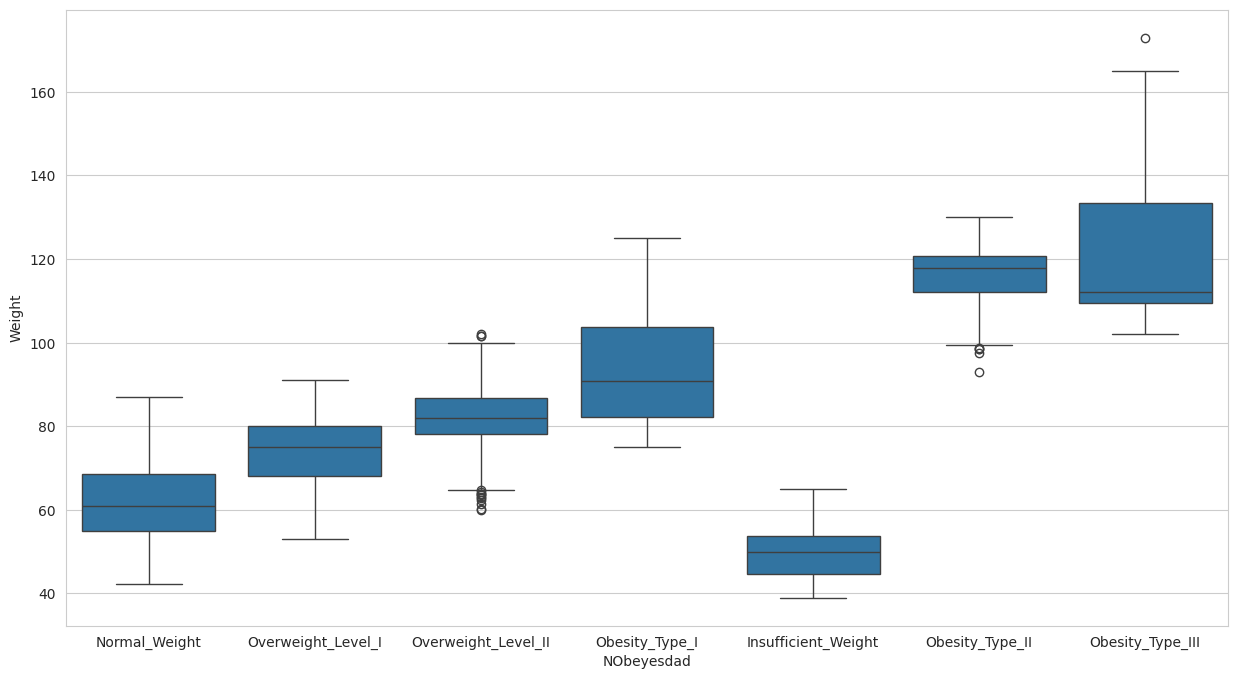
\includegraphics[width=0.4\textwidth]{boxplot.png}\label{fig:f2}}
      \caption{Exploratory Data Analysis Figures}
    \end{figure}
    Since weight is important and the values can have a wide range, we decided to use Min Max Scaling for all our data points to scale them in between a range of 0 and 1. This way the dataset's distribution will be preserved and when inputting the values into the various models, there won't be any overtly large numbers which is useful for stability when the model is training. (Figure 3)

    \subsection{Multilayer Perceptron}
        Our multi-level perceptron takes our input variables and links them to our first layer, with n nodes. For each node, the model performs the following: node($x$) = $\sum^n_{i=1}weight_{i,x} \times input_{i,x}$, where $n$ is the number of other nodes connected to x, $weight_{i_x}$ is the i-th connection to node x, and $input_{i,x}$ is the input being passed to the node through the i-th connection to node x. After we calculate these, we then go through each node and apply an activation function. This takes the input and returns a binary output based on the threshold we set for the perception. Then, we repeat this process for each layer of nodes, replacing the input layer with the layer we’ve just calculated. However, this process only works if we allow the perceptron to learn and adjust its weights. To do this, we compare the output we get, and adjust the weights accordingly, using a method known as backpropagation. We decided on using a 'Logistic' activation function and a 'Stochastic Gradient Descent' (SGD) learning algorithm, fine-tuned for our dataset by configuring a learning rate of 0.4 and a batch size of 100, to improve the model's learning potential. The architecture included two hidden layers with (17, 20) nodes, chosen to balance the trade-off between model complexity and the chance of overfitting. Since we pre-processed the data using 'MinMaxScaler' to transform the input features, it made the data more effective with the 'Logistic' activation function, as the logistic function is sensitive to larger input values due to outputs becoming either 0 or 1, where the gradients become very small. Following training and evaluation using 400 iterations, the MLP model was tested on our dataset. By the end, we found that our MLP model had an accuracy of 92.43\% in running our dataset. Although it is good, there is still room for improvement.
        
        After seeing the performance of our MLP, we decided to try and tune the hyperparameters to try and get better results and improve stability. We wanted to test many different combinations of layer sizes, layer amounts, activation functions, max iterations, and initial learning rates. Thus, we implemented a grid search to test all of these combinations and report back the optimal results. We ended up changing our hidden layer size to (20,24), learning rate to 0.3, and total number of iterations to 500. Ultimately, with the new parameters the accuracy increased to 93.38\% and the mean squared error reduced by 0.03 with a random state of 0 to keep it standardized, which was used in the pre-tuned MLP model as well.

    \subsection{Deep Neural Network}
    We also created a deep neural network as we thought it might do a better job of predicting classifications compared to the multilayer perceptron. The way a deep neural network works is very similar to a multilayer perceptron, but a deep neural network can have more hidden layers, helping it with more complex models. As the model was applied in sequence, with parts of 64 neurons and ReLU activation function for the first two layers. When using the softmax activation function in the output layer, the model provides a probabilistic interpretation of the classification in each of the seven weight classes. The model's predictions for each observation let us know how confident it is about its prediction. To stabilize our model, we trained the DNN model using 100 epochs and a batch size of 20. For the loss function, we used categorical cross entropy since it is used to measure the difference between the probability predicted from the softmax function and the probability from the actual class. We also used the dropout regularization technique where neurons are dropped out with a certain probability since the network will learn when only some of the neurons are still active, decreasing the likelihood of overfitting as the model has to adjust to the neurons being dropped out. Adding a dropout layer after each of the first two layers with a value of 0.5, where 50\% of the input will be dropped, led to a testing accuracy of 90.78\% and loss of .322. The training accuracy is around 97.27\% so the network performs pretty well with the testing set as the training accuracy is not much higher than the testing accuracy.
    \begin{figure}[h]
        \centering
        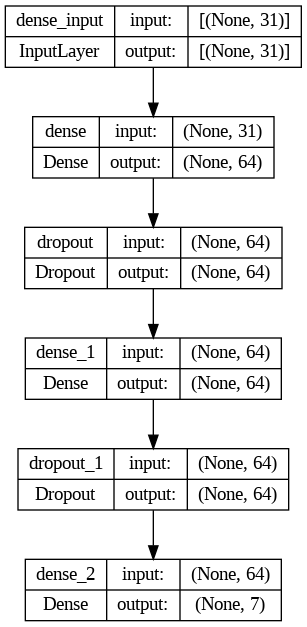
\includegraphics[width=0.2\linewidth]{model_plot.png}
        \caption{Deep Neural Network Visualization}
        \label{fig:enter-label}
    \end{figure}
    \subsection{eXtreme Gradient Boosting Model - XGBoost}
    Finally, we also created an extreme gradient boost model, which we thought would be useful for comparison since it takes a different approach than our multilayer perceptron and deep neural network. While those create nodes and layers, the extreme gradient boost model creates a decision tree, which creates leaves and branches to ultimately predict what classification data should fall under. It builds its model by iteratively correcting the errors in the previous decision tree. This way the model progressively gets better during training. With the XGB model, we ran it initially with the 'multi:softprob' loss function which provides the probability of the data being in each of the output classes. We also split the dataset into 3 parts with a training, test, and validation with a split of 80:10:10 respectively. Since we knew from the literature review that XGBoost would perform really well, we used a validation dataset in training and tracked its classification error with hopes of preventing overfitting. After running the initial model, the accuracy for the testing set was 97.15\% which was around what we expected as from the literature review they got around 98\%. Then we plotted the classification error for both the training and the validation set against the number of epochs which is shown below. From this figure, we can see that the validation set doesn't have huge improvements past 40 epochs, which is a perfect opportunity to use early stopping. 
    \begin{figure}[h]
      \centering
      \subfloat[Without Early Stopping]{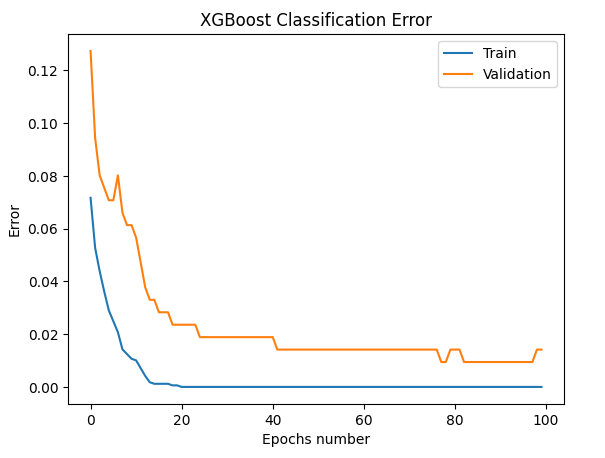
\includegraphics[width=0.4\textwidth]{firstpic.png}\label{fig:f1}}
      \hfill
      \subfloat[With Early Stopping]{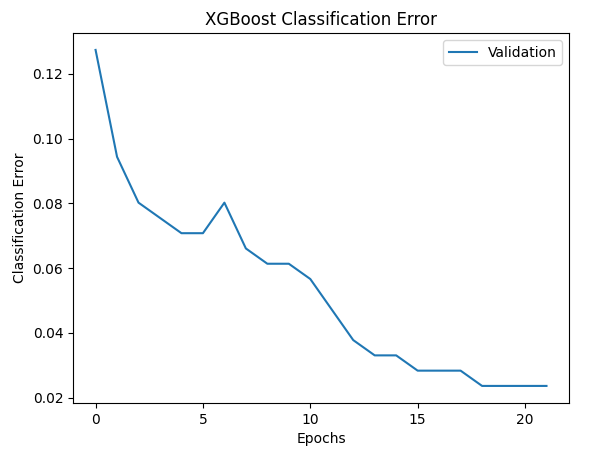
\includegraphics[width=0.4\textwidth]{second_pic.png}\label{fig:f2}}
      \caption{XGB Early Stopping}
    \end{figure}
    
    Early stopping is an overfitting technique that stops training after a certain number of iterations where the validation dataset performance does not improve. In our case, we want the model to stop training at any point between 20 and 40 epochs, because after that range there are no improvements on the graph. We then created an optimized version of the XGBoost model with an early stopping rounds value of 3 which is the number of consecutive rounds of no improvement needed for the model to stop training. The value is typically chosen by taking 10\% of the number of epochs we want to train, which is between 20 and 40, so in this case the model would stop after 3 iterations of no improvement if we take 30 as the average. After running this early stopping version, we got 97.63\% as the test accuracy, which when looking at the validation set error against the number of epochs figure makes sense as the model stopped after 21 iterations and didn’t improve for the last 3 iterations which is our signal to stop. From this, we can conclude that the early stopping version of the XGB has reduced the possibility of overfitting from our first XGBoost model and is a strong contender for our best model.

    \subsection{Cross Validation on the Models}
    For our three models, we performed a k-fold cross-validation, which creates a model using a new, randomized test/train split for each k-fold. We can see how the models perform on different subsets of the data, and the one that performs the best on all different folds will be the most generalizable model. Afterwards, we can find the average accuracy for each model using the following: $\frac{1}{k}\sum^k_{i=1}$accuracy($iter_i$), where $k$ is the number of iterations, and $iter_i$ is the i-th iteration of the k folds. In our case, we decided on 10 iterations of k-fold, as it was double the default value we saw most functions use. Doubling it would allow us to gain more information on how our models performed on average, without causing too much stress from creating models. 

\section{Results}

\begin{table}[h]
    \centering
    \begin{tabular}{|c|c|c|c|c|}
         \hline
         Type of Model & Accuracy & Precision & Recall & CV Accuracy\\
         \hline
         Optimal MLP & 93.38\% & 94\%  & 93\% & 91.58\%\\
         \hline
         DNN & 90.78\% & 91.35\% & 89.83\% & 92.55\%\\
         \hline
         XGB Early Stopped & 97.63\% & 97.63\% & 97.63\% & 95.03\%\\
         \hline
    \end{tabular}
    \caption{Compares the three models with different measures}
    \label{tab:my_label}
\end{table}
    Here is the list of metrics used in evaluation:
    \begin{enumerate}
        \item Accuracy - We want to see how well the model correctly classifies people into a class.
        \item Precision - We want to know for each class, how many of the predictions were actually truly in that class (factors in false positives)
        \item Recall - We want to know for each class, how well the model reduces the number of false negatives.
        \item Average Accuracy from Cross Validation - Check how well the model works on different subsets of the dataset for generalization
    \end{enumerate}
    
    In addition to accuracy being factored, precision and recall are important as well since they emphasize how much the model falsely classifies data. In the case of a false classification, if a person should be classified into Obesity Level II, but the model classifies them into Overweight Level II, there may be a difference in the urgency of their response towards that classification. Overweight Level II is still a problem, but not as alarming as Obesity Level II, so they might not take action, which can lead to health problems since the person is actually obese. 

    We ultimately found that our XGBoost model with Early Stopping had the highest accuracy out of all of the other models that we created and performed better in all other metrics including precision, recall, and the average accuracy from cross validation. The deep neural network also had great accuracy, precision, and recall but was not as good as our extreme gradient boost model. The loss function of the neural network was also fairly high even with dropout regularization, which is not great. Finally, we found that our multi-layer perceptron had good performance across the board, but still not as good as the XGBoost. We don’t find these results super shocking, since the papers we looked at the literature review all had models with high accuracy and the XGBoost model was the consistent best model displaying extremely high accuracy. Beyond that, it is a little surprising that the linked-node neural networks performed worse than the extreme gradient boost given some of the linear trends we saw in the data, especially between obesity and weight. Overall, we feel confident in concluding that the XGBoost with Early Stopping was the best model since it checks for overfitting and also performs extremely well across the board compared to the other models. 
\section{Conclusion and Discussion}
Obesity is a looming issue around the world that continues to worsen each year. It can cause many serious health problems including stroke, diabetes, and high blood pressure. It is crucial that people know what obesity classification level they are in to help take preventative measures before the problem worsens. If they know and understand the severity of their health situation, they are more likely to change their eating habits and make the necessary lifestyle changes to become a healthier person. To achieve this goal we used three different machine learning models which include the multi-layer perceptron (MLP), deep neural network (DNN), and extreme gradient boosting classifier (XGBoost). Each of these models performed well on the testing dataset with the XGBoost classifier standing out with 97.63\% accuracy and 95.03\% average accuracy from cross validation to ensure the model works well with any subset of the data. The XGBoost model also utilized Early Stopping to reduce the likelihood of overfitting; the model would run on a limited amount of epochs rather than all of the epochs since past a certain point, the model would not improve. We connected this model to our frontend which takes in user input in a survey-like fashion and outputs their weight level as well as personalized feedback based on provided answers. 

For future work, there are many possibilities to improve our project beyond obesity level classification. For example, by incorporating other datasets into our obesity level classifier, we can create personalized exercise and nutrition plans for those seeking healthy lifestyle changes. Additionally, we could utilize a hybrid or ensemble approach to introduce more models, which would further enhance the accuracy of our classifier. Also, since the dataset was only taken from 3 countries, we are unable to generalize the dataset across the globe, which may be a point of interest in the future.

In conclusion, we hope that this project can help people better understand their health and feel empowered to make the necessary changes to live a longer, healthier life. 

\newpage
\section{References}

\begin{enumerate}
    \item Searles, M. (2024, March 1). Obesity now greater risk to global health than hunger. The Telegraph. https://www.telegraph.co.uk/news/2024/03/01/obesity-now-greater-risk-global-health-hunger-lancet-study/
    \item World Obesity Day Atlases | Obesity Atlas 2023. (2023). World Obesity Federation Global Obesity Observatory. https://data.worldobesity.org/publications/?cat=19
    \item Centers for Disease Control and Prevention. (2022, July 15). Consequences of Obesity. Centers for Disease Control and Prevention; CDC. https://www.cdc.gov/obesity/basics/consequences.html
    \item Estimation of Obesity Levels Based On Eating Habits and Physical Condition . (2019). UCI Machine Learning Repository. https://doi.org/10.24432/C5H31Z.
    \item World Obesity Federation Global Obesity Observatory. (n.d.). World Obesity Federation Global Obesity Observatory. Retrieved March 15, 2024, from https://data.worldobesity.org/\#MX
    \item Kaur, R., Kumar, R., \& Gupta, M. (2022). Predicting risk of obesity and meal planning to reduce the obese in adulthood using artificial intelligence. Endocrine, 78(3), 458–469. https://doi.org/10.1007/s12020-022-03215-4
    \item Akash Choudhuri. (2022). A Hybrid Machine Learning Model for Estimation of Obesity Levels. MedRxiv (Cold Spring Harbor Laboratory). https://doi.org/10.1101/2022.08.17.22278905
    \item Forte, P., Encarnação, S., Monteiro, A. M., Teixeira, J. E., Hattabi, S., Sortwell, A., Branquinho, L., Amaro, B., Sampaio, T., Flores, P., Silva-Santos, S., Ribeiro, J., Batista, A., Ferraz, R., \& Rodrigues, F. (2023). A Deep Learning Neural Network to Classify Obesity Risk in Portuguese Adolescents Based on Physical Fitness Levels and Body Mass Index Percentiles: Insights for National Health Policies. Behavioral Sciences (Basel, Switzerland), 13(7), 522. https://doi.org/10.3390/bs13070522
    \item World Health Organization. (2024, March 1). Obesity and overweight. World Health Organization. https://www.who.int/news-room/fact-sheets/detail/obesity-and-overweight
    \item Palechor, F.M., \& Manotas, A.D. (2019). Dataset for estimation of obesity levels based on eating habits and physical condition in individuals from Colombia, Peru and Mexico. Data in Brief, 25.
\end{enumerate}

\newpage
\section{Project Roadmap} 





\begin{enumerate}
    \item Describing the problem scientifically\\
    \emph{Completed by Week 4}
        \begin{itemize}
            \item Gathered statistics from sources like the World Obesity Atlas projecting a significant rise in global obesity rates.
            \item Found various adverse health impacts of obesity, including increased risks of chronic diseases such as diabetes, heart disease, and mental illness.
        \end{itemize} 

    \item Background study(literature review or related work) \\
    \emph{Completed by Week 4}
    \begin{itemize}
        \item Analyzed papers like “Obesity Prediction using Ensemble Machine Learning Approaches,” “Machine Learning Approach for the Early Prediction of the Risk of Overweight and Obesity in Young People,” and “A machine learning approach for obesity risk prediction”
        \item Gained insights regarding machine learning techniques, MLP models, and comparative analysis for obesity prediction 
    \end{itemize}
    
    \item Dataset: Understanding and Exploratory Data Analysis \\
    \emph{Completed by Week 5}
    \begin{itemize}
        \item Utilized visualizations like correlation matrices, pairplots, and boxplots to identify key patterns
        \item Identified strong correlations between target variable (NObeyesdad) and other variables, with weight showing the most significant influence across multiple obesity levels.
    \end{itemize} 
    
    \item Developing Accurate Prediction Model(s) \\
    \emph{Completed by Week 6}
    \begin{itemize}
        \item Multi-Level Perceptron (MLP): Utilized a two layer model with sizes 17 and 20, a logistic activation function, and optimized hyperparameters through grid search cross validation 
        \item Deep Neural Network (DNN): Constructed a model of 3 dense layers and 2 dropout layers, as well as a softmax activation function. 
Extreme Gradient Boost (XGBoost): Implemented with gradient boosting decision trees and soft prob loss function. 
    \end{itemize}
    
    \item Evaluation of the model(s) and Testing the performance \\
    \emph{Completed by Week 7}
    \begin{itemize}
        \item Model performance evaluated using 10-fold cross validation
        \item XGBoost performed the best, DNN performed well, and MLP performed the poorest
    \end{itemize}
    
    \item Developing a basic web-based front-end to invoke and run the model(s) on input data and display the prediction output \\ 
    \emph{Completed by Week 8}
    \begin{itemize}
        \item Created a front end using Streamlit, allowing users to input values for the features and receive an obesity level classification based on the XGBoost model.
    \end{itemize}
     
    \item Prepare the presentation and finalize the paper to be ready for submission \\ 
    \emph{Completed by Week 9}
    \begin{itemize}
        \item All the project deliverables, including the presentation and research paper, are finalized and ready for submission before the deadline. 
    \end{itemize}

\end{enumerate}


\end{document}
